\documentclass[12pt,oneside,a4paper]{article}

\usepackage[utf8]{inputenc}
\usepackage[document]{ragged2e}

\usepackage{times} % Use the Times New Roman font

\usepackage[brazilian]{babel}
\usepackage[margin=1in]{geometry}
\usepackage{natbib}
\usepackage{graphicx}
\usepackage{float}
\usepackage{amsmath}
\usepackage{setspace}

\begin{document}

\begin{titlepage}
\enlargethispage{\footskip}
\setlength{\parindent}{0pt}

\begin{center}
    \onehalfspacing
    \Large Universidade Federal de Minas Gerais
    \\ Departamento de Ciência da Computação
    
    \vspace{80mm}
    
    \Large{DCC057 Mineração de Dados}
    \\ \Large \textbf{Trabalho Prático 3 --- Relatório de Descrição dos Dados}
    
\end{center}

\vspace{\fill}

\begin{minipage}[b]{\textwidth}
    \centering
    \onehalfspacing
    \large
    Alexander Thomas Mol Holmquist \\
    16 de março de 2021

\end{minipage}

\end{titlepage}

\justify

\section{Objetivo}

Este relatório tem como objetivo clarificar aspectos sobre a descrição dos dados, principalmente em vista do plano inicial do projeto.

\section{Percepções}

Rapidamente ficou claro que os passos delineados pelo plano inicial do projeto são fruto de inexperiência com mineração de imagens. Por exemplo, é dito no plano inicial, como recomendação para o passo 1 da segunda fase, que deve-se gerar métricas como a média, variância, etc. Porém, isto não é interessante para imagens, porque o número de atributos é grande demais para permitir que uma análise individualizada dos dados seja feita..

Outro equívoco foi recomendar a produção de uma figura ilustrando o banco de dados de dimensionalidade reduzida, especificamente de duas dimensões. Novamente, se durante o desenvolvimento de tal plano, houvesse um entendimento básico da forma de um banco de dados de imagens, este passo não teria sido recomendado. A razão é a mesma do item anterior. Não é possível condensar uma imagem, que tem milhares e milhares de atributos, em poucos componentes principais.

\section{Resultados}

Apesar das falhas mencionadas, foi possível gerar duas saídas úteis para o projeto.

\begin{enumerate}
    \item Proporção de imagens de câncer benigno e maligno
    \begin{figure}[h!]
        \centering
        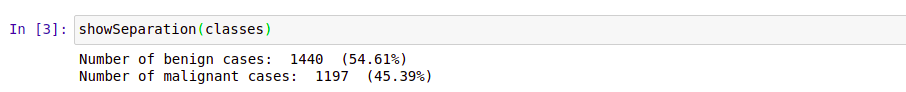
\includegraphics[width=15cm]{notebook-fase-2-show-separation.png}
        \caption{Proporção benigno/maligno}
        \label{fig:my_label}
    \end{figure}
    
    \item Exemplo de imagem para ambos os casos
    \begin{figure}[h!]
        \centering
        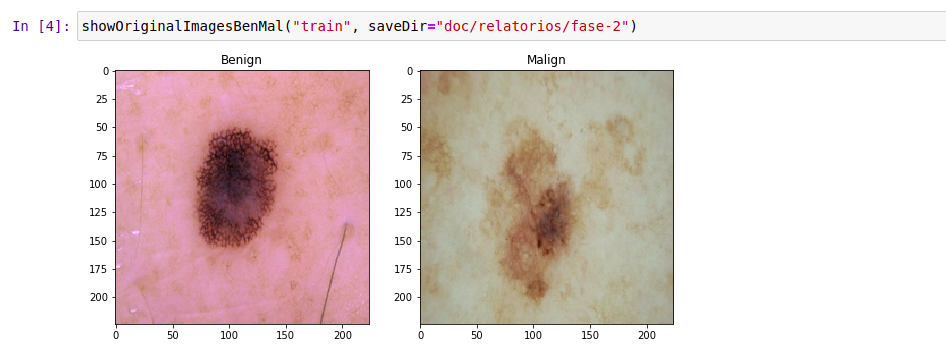
\includegraphics[width=15cm]{notebook-fase-2-show-ben-mal.png}
        \caption{Exemplos de imagem para cada caso}
        \label{fig:my_label}
    \end{figure}
\end{enumerate}

Esta última imagem com os dois casos foi também salvo no diretório "doc/relatorios/fase-2", junto com o presente relatório.

\clearpage

\end{document}
